\section{Problem Description}

The lab setup consist of a base with a movable arm as seen in \cref{fig:heli_setup}. The arm has a balancing weight in one end and a helicopter with two rotors on the other end. By having a different thrust one can move the pitch of the helicopter and thus also move the travel of the helicopter We can derive simple set of differential equations to describe the system:

\begin{subequations}
    \begin{gather}
        \ddot p=K_1V_d, \ \  K_1=\frac{K_fl_h}{J_p}\\
        \ddot\lambda = -K_2p, \ \  K_2=\frac{K_pl_a}{J_t}\\
        \ddot e =K_3 V_s-\frac{T_g}{J_e}, \ \  K_3=\frac{K_fl_a}{J_e}
    \end{gather}
\end{subequations}

Furthermore, we want to stabilize the system by adding a PD controller to the pitch and a PID controller to the elevation. This yields the model equations \cref{eq:model_al}.

\begin{subequations}\label{eq:model_al}
	\begin{align}
    \ddot{e} + K_3 K_{ed}\dot{e} + K_3 K_{ep} e &= K_3 K_{ep} e_c \\
		\ddot{p} + K_{1} K_{pd} \dot{p} + K_{1} K_{pp} p &= K_{1} K_{pp} p_{c} \label{eq:model_se_al_pitch} \\
		\dot{\lambda} &= r \label{eq:model_se_al_lambda} \\
		\dot{r} &= -K_{2} p \label{eq:model_se_al_r}
	\end{align}
\end{subequations}

\begin{figure}[h]
    \centering
    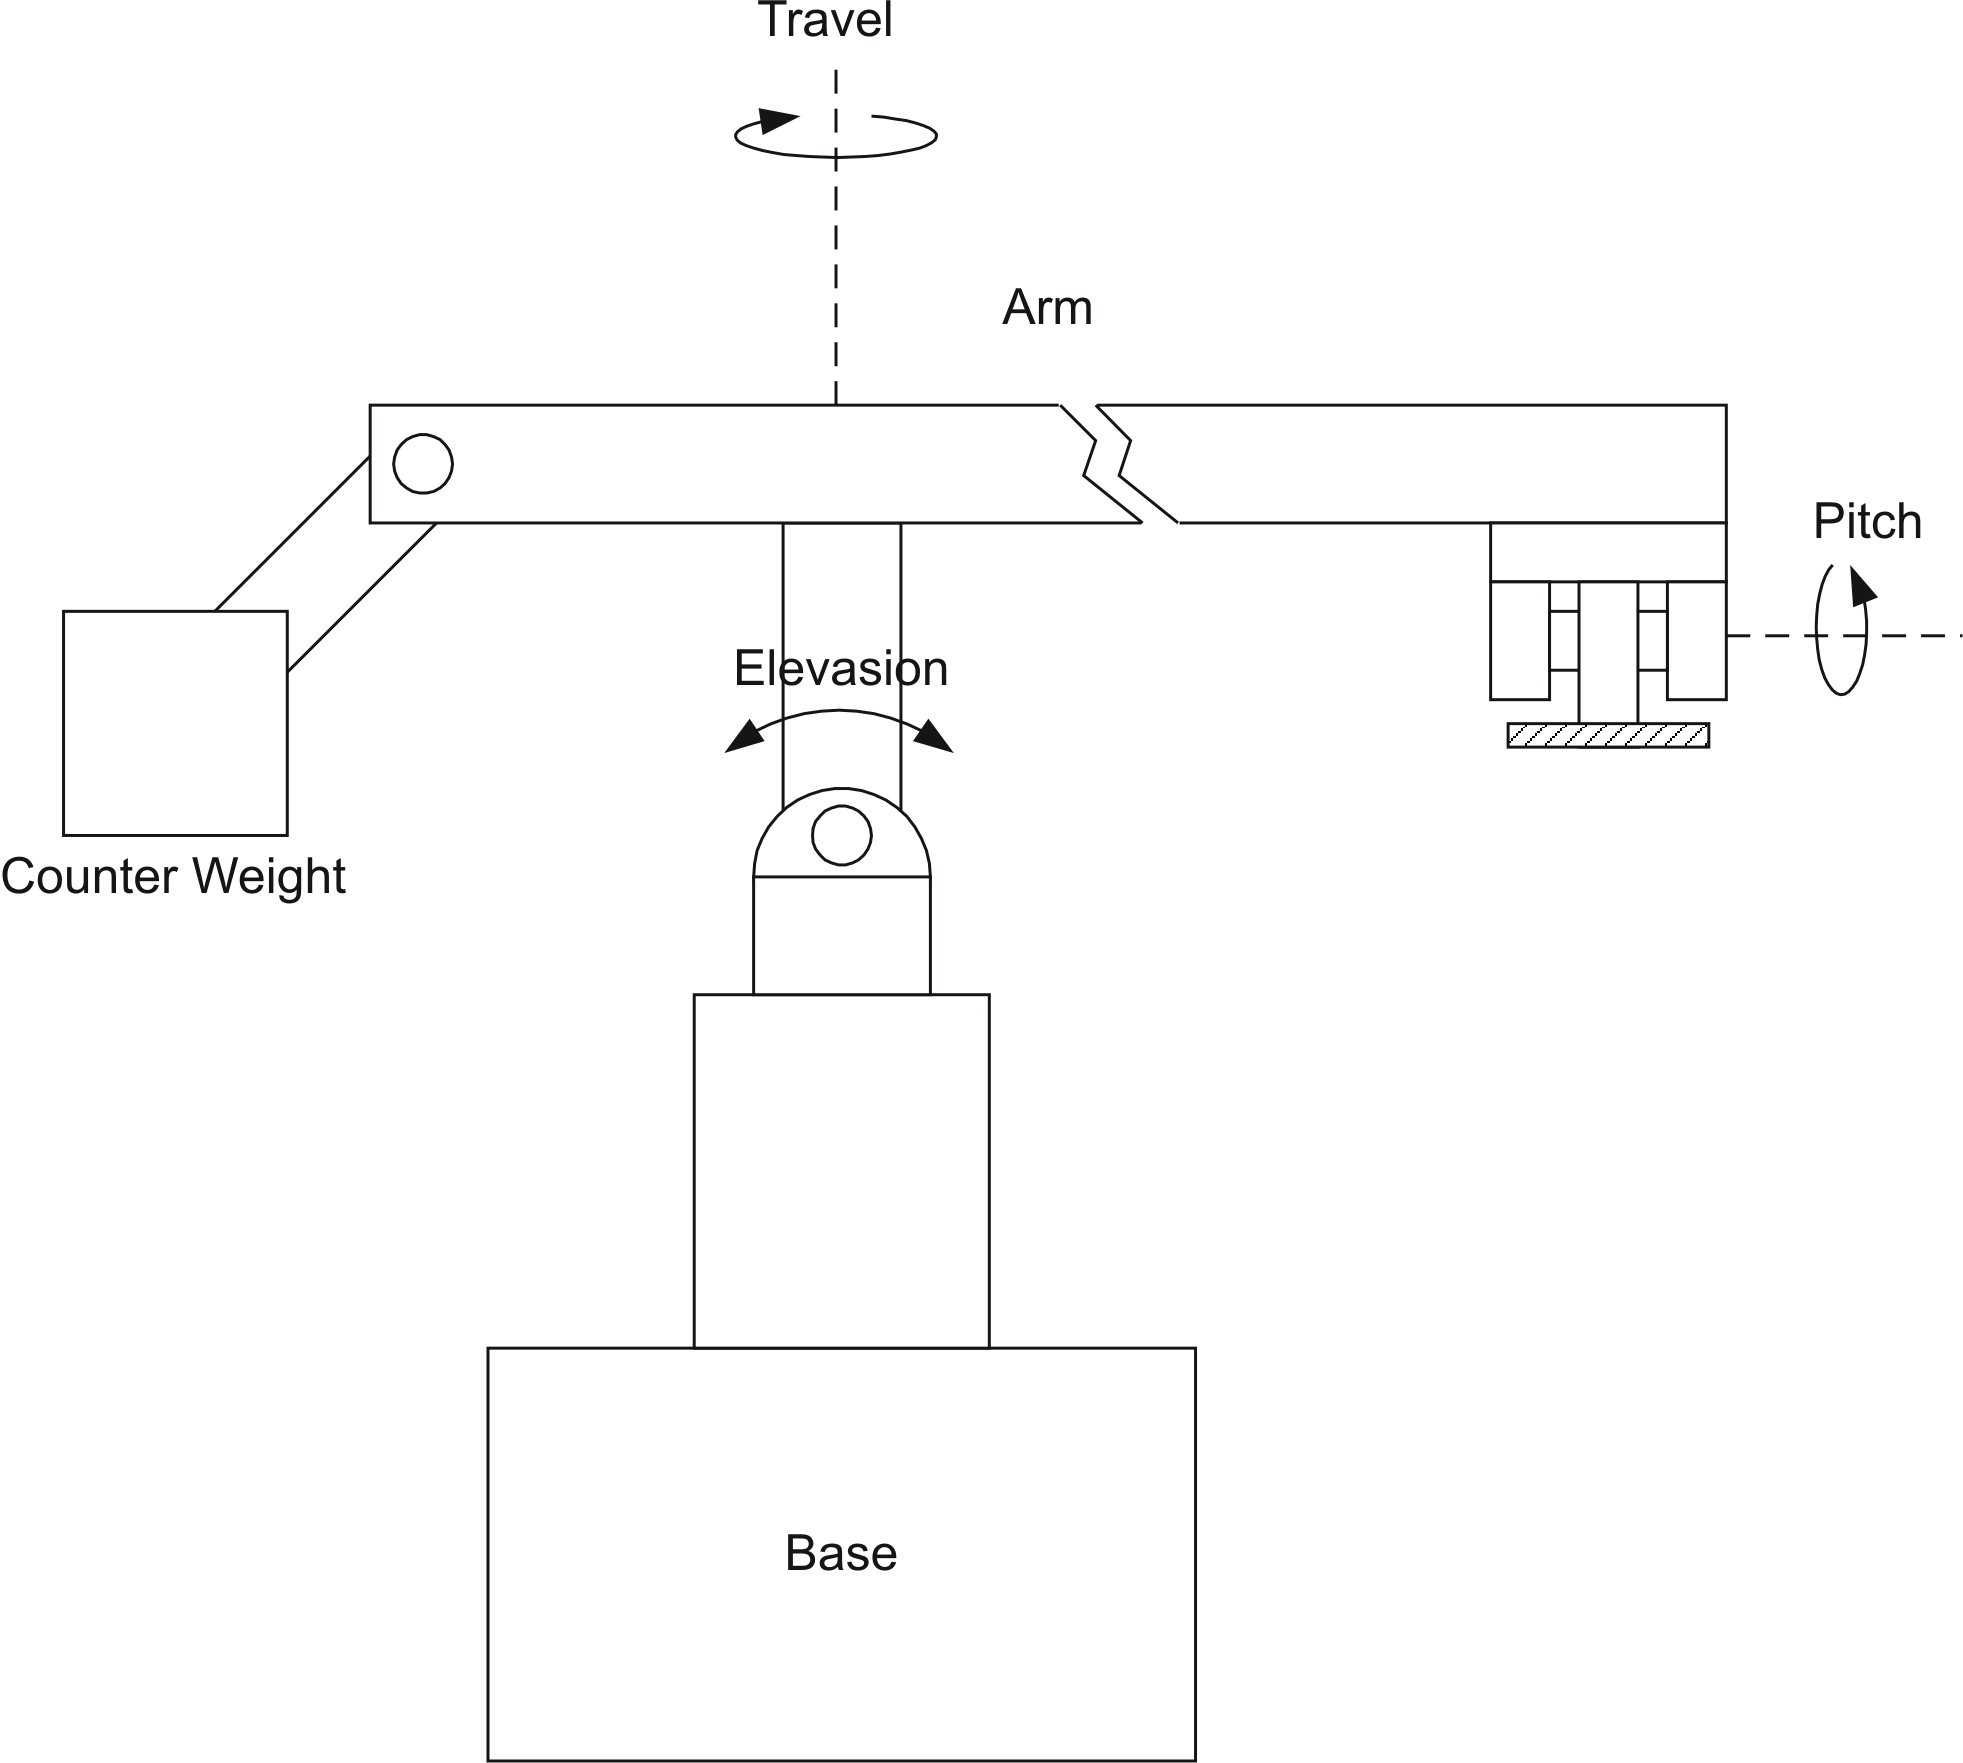
\includegraphics[width = 0.65\textwidth]{fig/lab_setup.png}
    \caption{Illustration of lab helictoper setup (courtesy of \cite{Assignment-text})}
    \label{fig:heli_setup}
\end{figure}
